\chapter*{Meshes}

\newpage
\section{cube_fiber_2d.geo}

\begin{figure}[!hht]
  \centering
  \resizebox{10cm}{!}{
  \includegraphics[width=0.5\textwidth]{figures/cube_fiber_2d.pdf}
  %\caption{A picture of the same gull looking the other way!}
  }
\end{figure}

\begin{figure}[!hht]
  \centering
  \resizebox{10cm}{!}{
  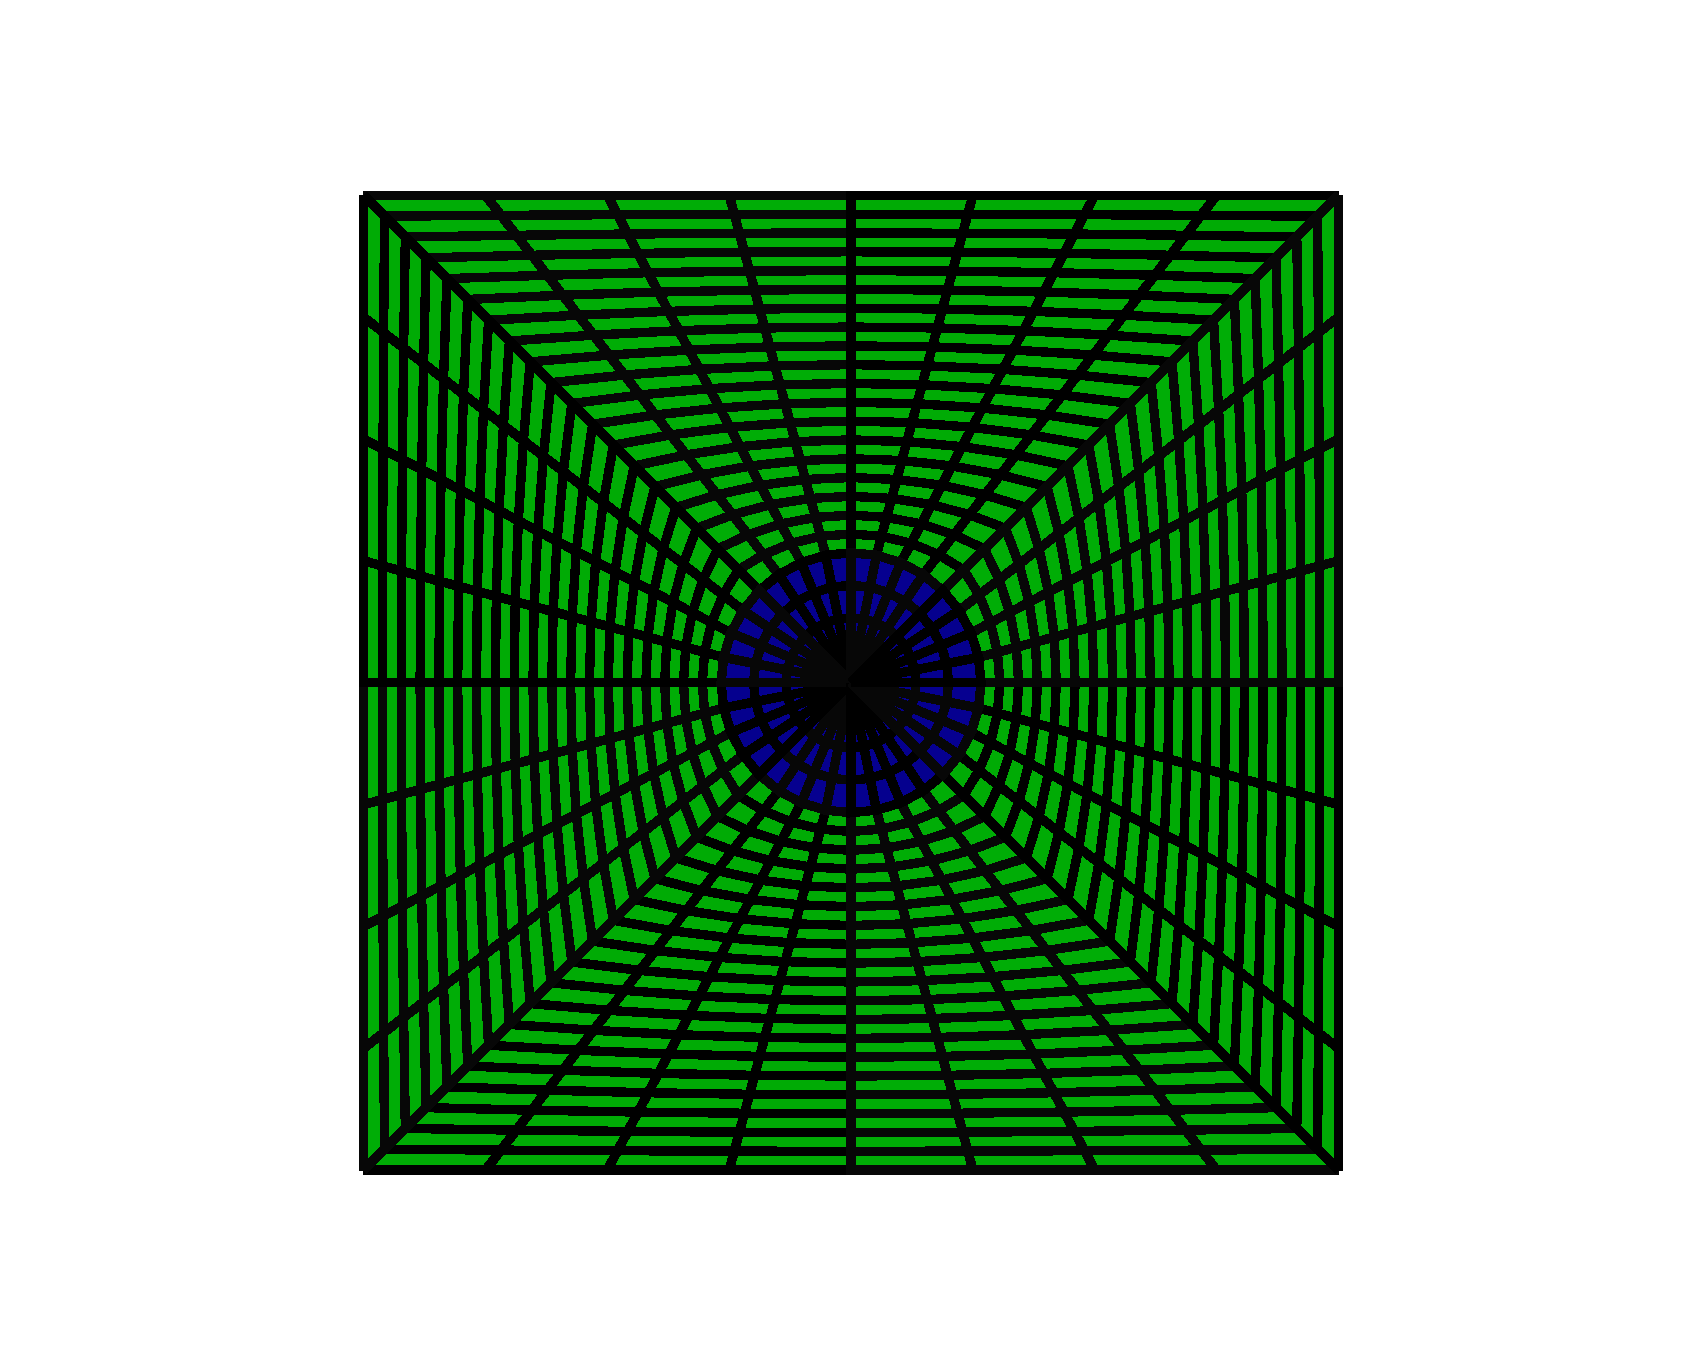
\includegraphics[width=0.5\textwidth]{figures/cube_fiber_2d_msh.pdf}
  %\caption{A picture of the same gull looking the other way!}
  }
\end{figure}

\newpage
\section{fiber_dev_2d.geo}

\begin{figure}[!hht]
  \centering
  \resizebox{10cm}{!}{
  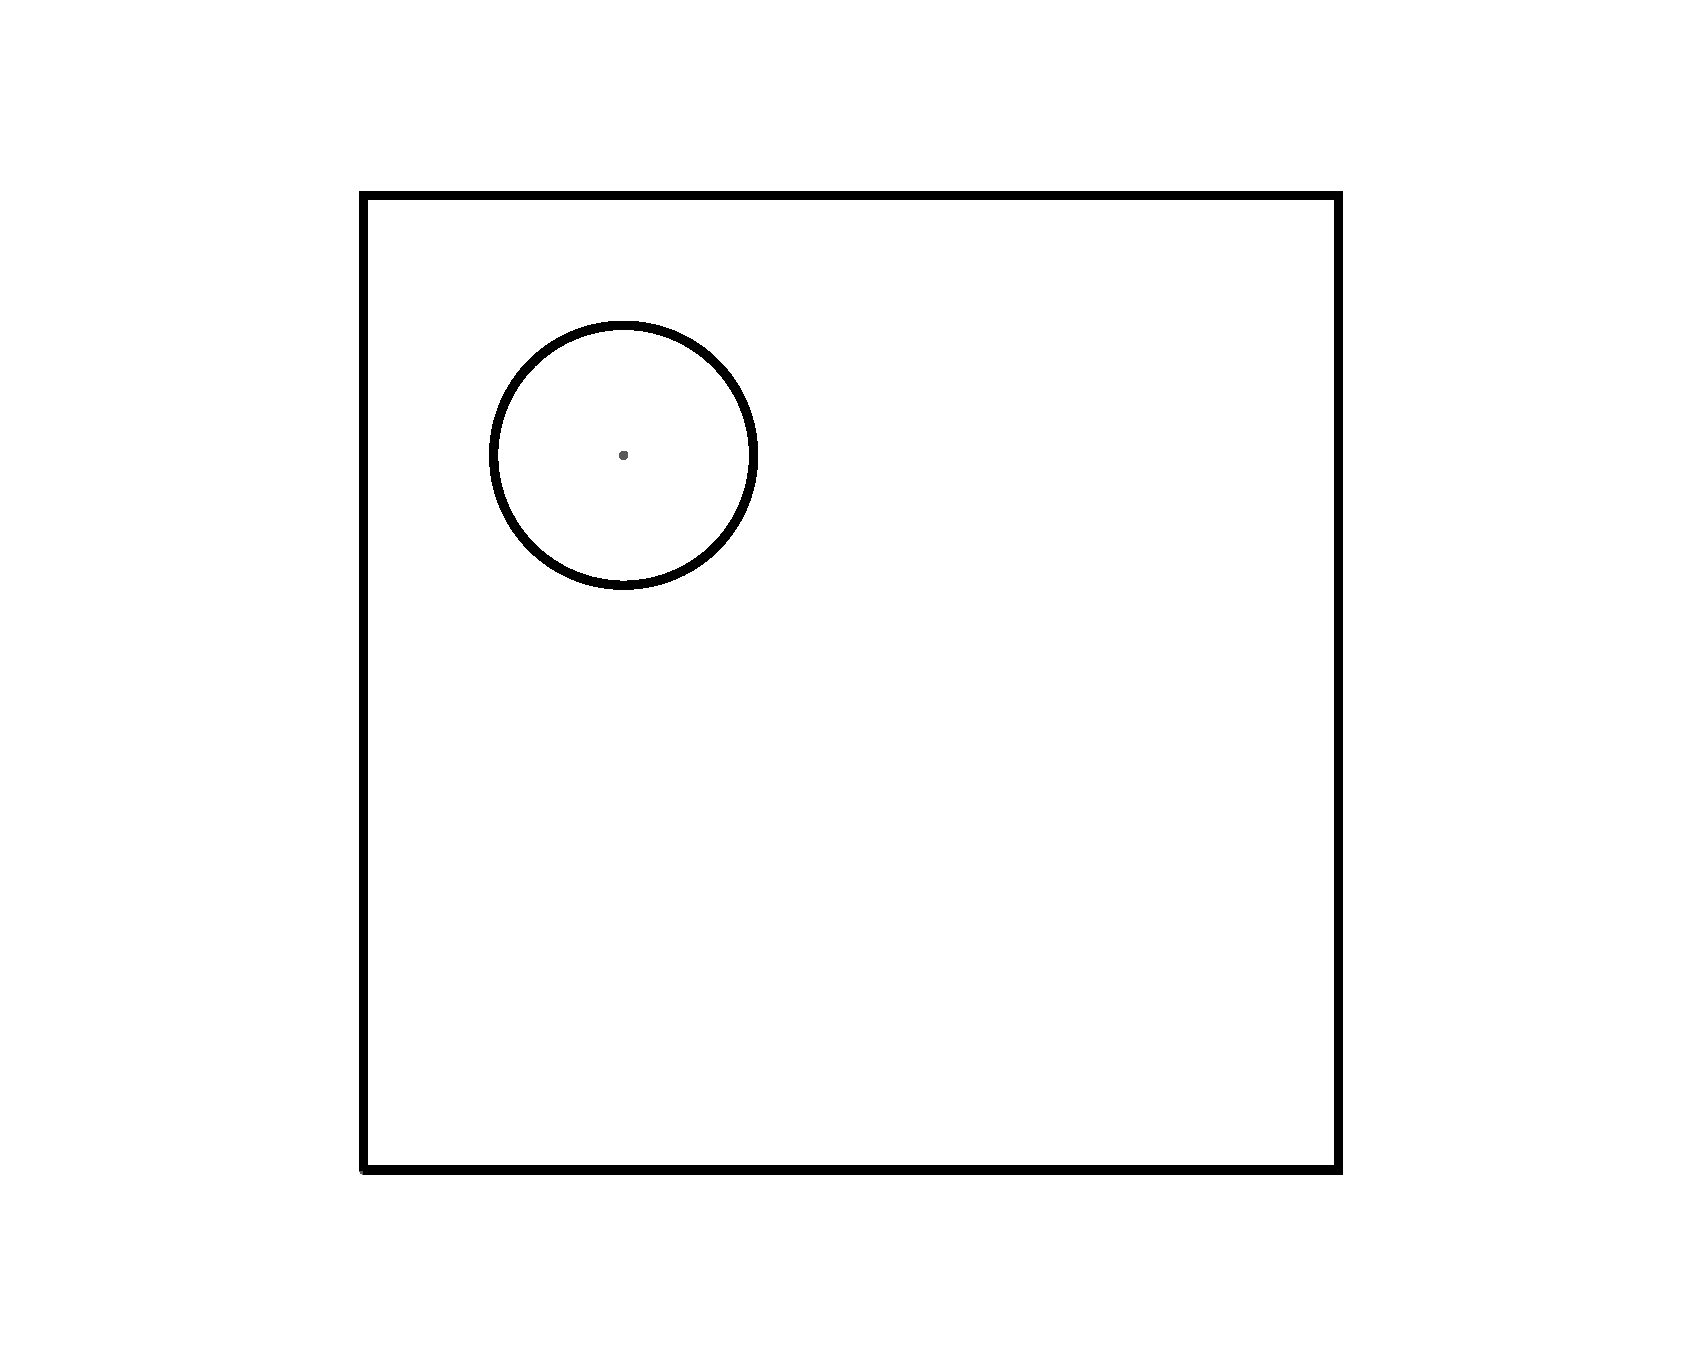
\includegraphics[width=0.5\textwidth]{figures/fiber_dev_2d_geo.pdf}
  %\caption{A picture of the same gull looking the other way!}
  }
\end{figure}

\begin{figure}[!hht]
  \centering
  \resizebox{10cm}{!}{
  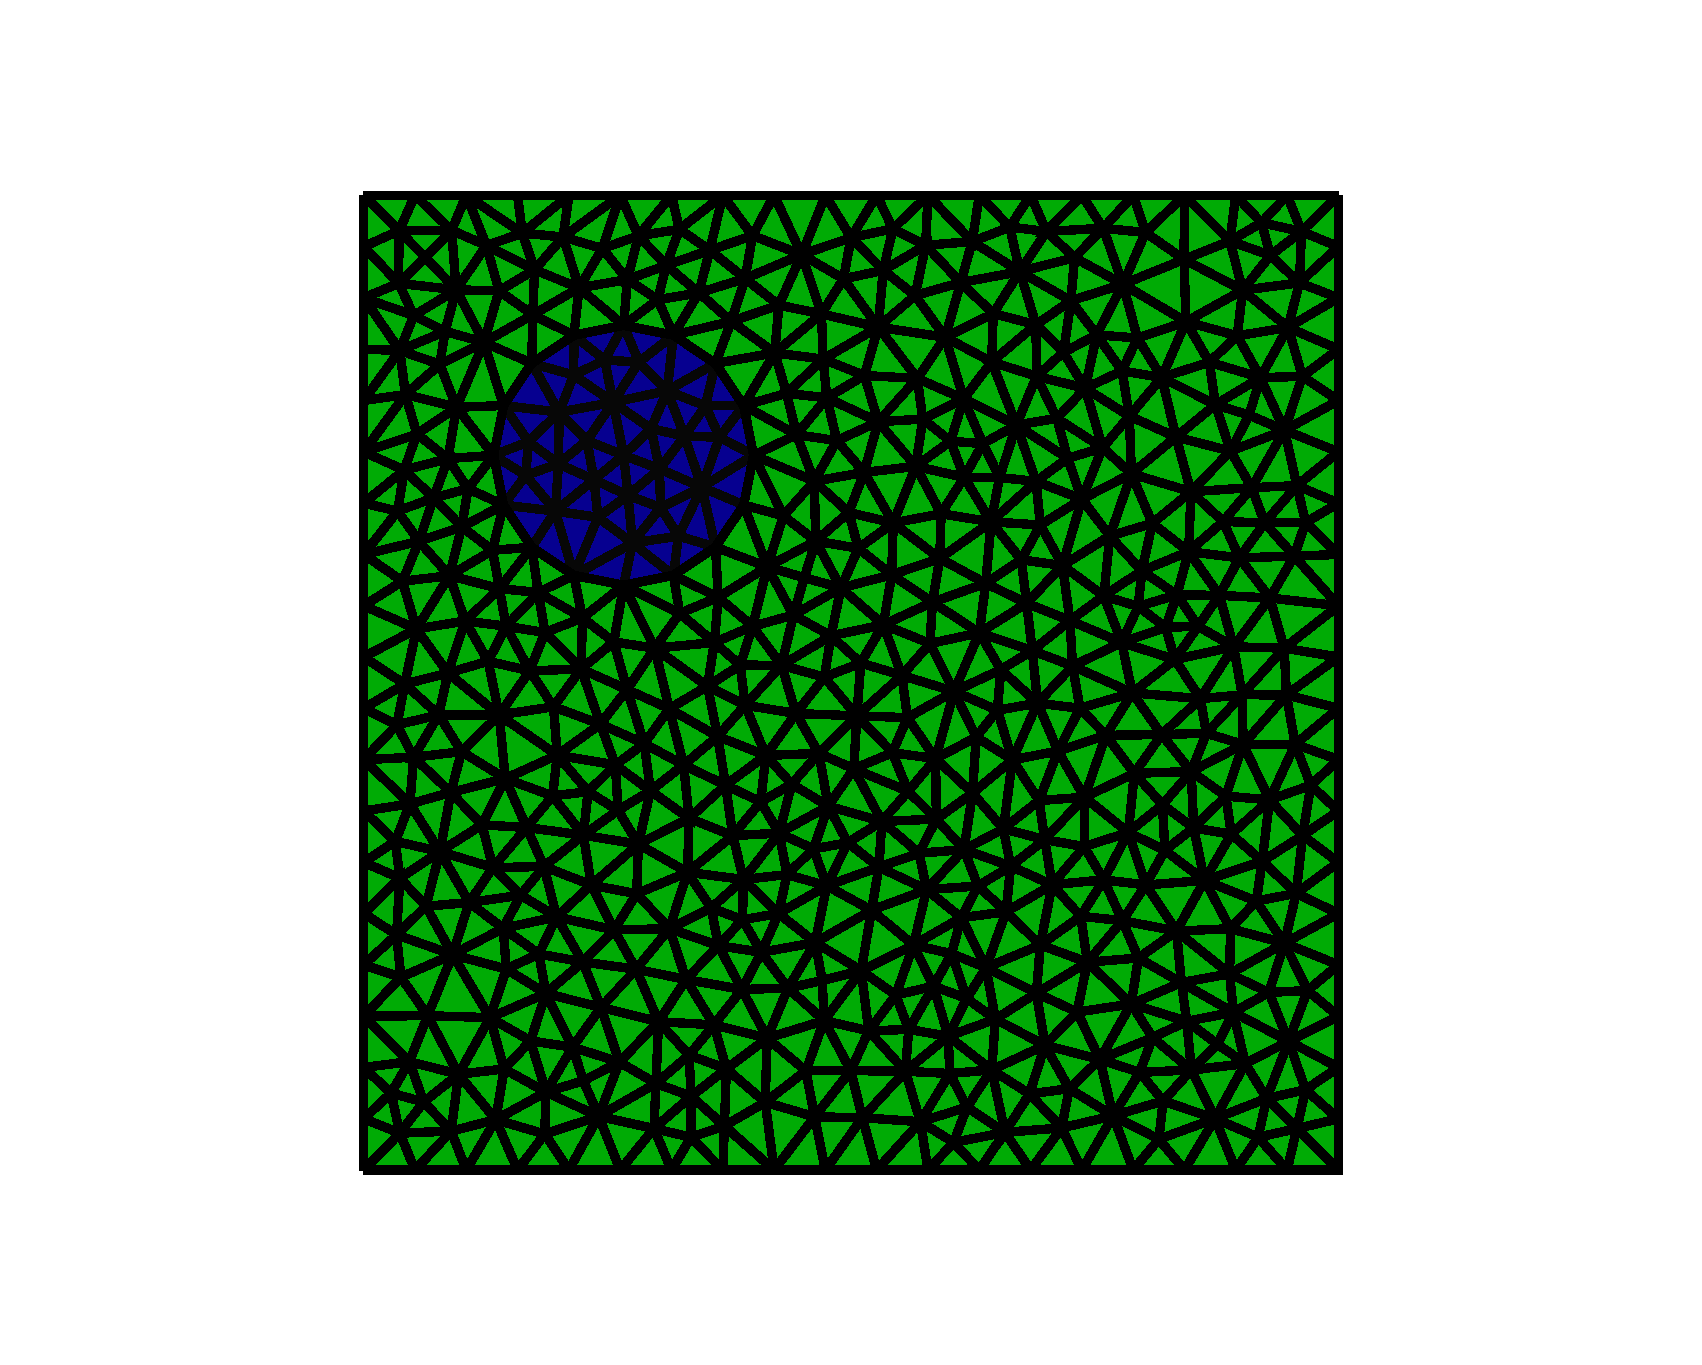
\includegraphics[width=0.5\textwidth]{figures/fiber_dev_2d_msh.pdf}
  %\caption{A picture of the same gull looking the other way!}
  }
\end{figure}

\newpage
\section{fiber_tr_2d.geo}

\begin{figure}[!hht]
  \centering
  \includegraphics[width=0.5\textwidth]{figures/fiber_tr_2d.pdf}
  %\caption{A picture of the same gull looking the other way!}
\end{figure}

\begin{figure}[!hht]
  \centering
  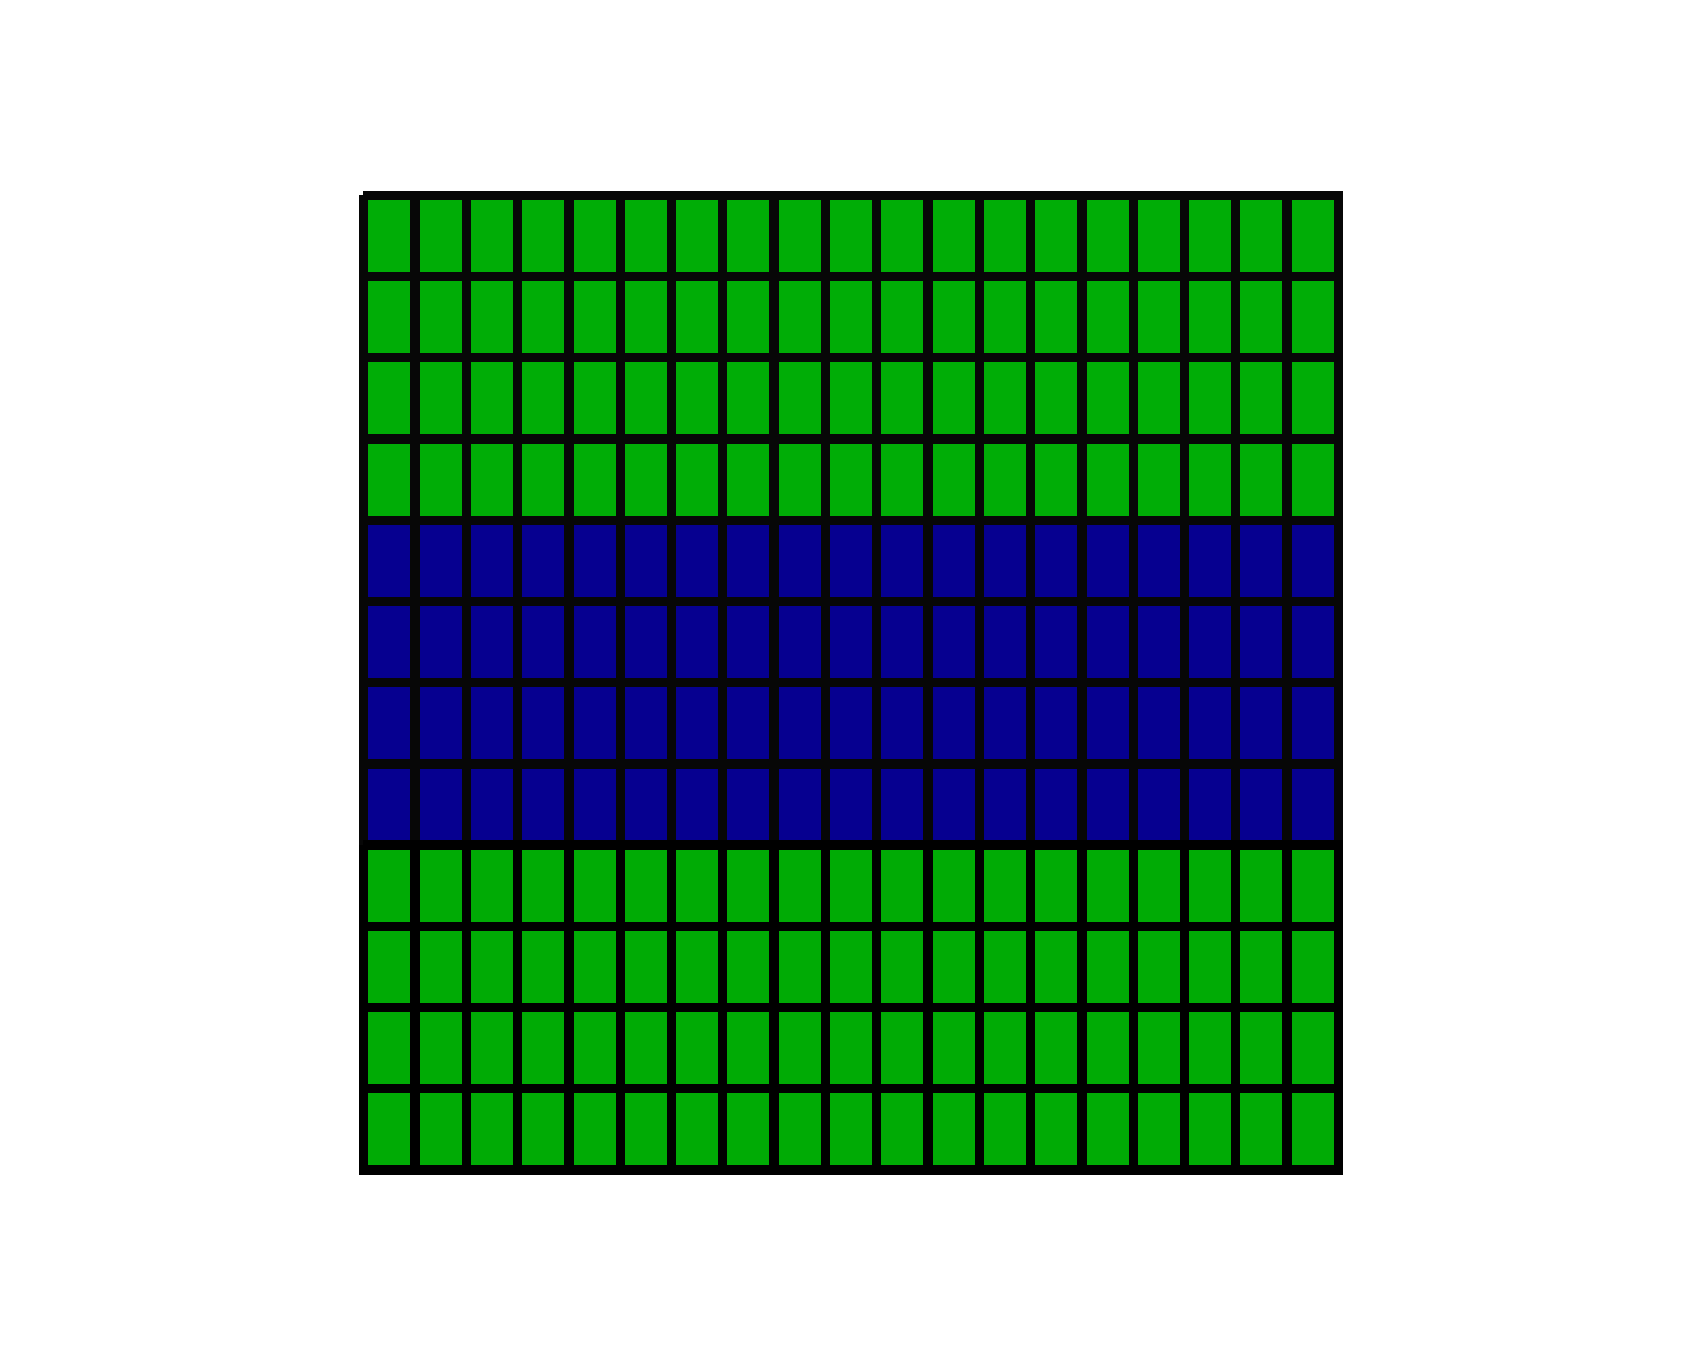
\includegraphics[width=0.5\textwidth]{figures/fiber_tr_2d_msh.pdf}
  %\caption{A picture of the same gull looking the other way!}
\end{figure}

